\documentclass{article}
\usepackage{graphicx}
\usepackage{fullpage}
\begin{document}

\title{Fire Dynamics Repository}
\author{M. Currie and B. Quaife}
\maketitle

%\abstract

%This document is meant to make sense of the plots, movies, and scripts located in this repository. The discussions in this document will be organized into four sections: 1) real infrared image data, 2) dynamic mode decomposition (DMD) for the real IR data, 3)  cellular automata (CA) to model the spread of fires, and 4) fire box data, results, etc.

%\pagebreak
\section{Real IR Data}
There are three real data sets that we are working with in the subsequent analyses. 
The datasets are designated 13fsingle1, 13fsingle2, and 13fsingle3, however 
henceforth they shall be referred to as Fire 1, Fire 2, and Fire 3, respectively. Here we 
present basic statistics for each of the three datasets. It is important to note that all 
temperatures are in Celsius.

All of the datasets were reduced from their original forms to get 
rid of frames where there was significant readout noise and frames
where nothing was happening (e.g. frames where the fire had already
passed: static frames). The frame numbers used are specified in each respective section

\begin{table}

\begin{tabular}{|c|c|c|c|c|c|c|}
\hline
 & Mean Temp & Median Temp & Std Dev & Max Temp & Min Temp & Timestep (s) \\
\hline
Fire 1 & 301.939 & 221.310 & 128.379 & 890.108 & 199.998 & 1.000 \\
\hline
Fire 2 & 218.188 & 159.911 & 137.907 & 921.466 & 99.9974 & 1.000 \\
\hline
Fire 3 & 267.044 & 199.998 & 113.061 & 849.827 & 199.998 & 1.000 \\
\hline
\end{tabular}
\centering
\caption{This table shows some basic values for each of the fires. These are overall values, meaning that it looks at all data from all timesteps.}
\end{table}

\subsection{Fire 1}


\begin{table}
\centering
\begin{tabular}{|c|c|}
\hline
Data range used & Frames 60 through 300 \\
\hline 
               & 32, 72, 115, 136, 137, 156, 177, 197, 217, 238, \\
               & 258, 278, 298, 318, 339, 359, 379, 399, 420, 459,\\
Garbage frames & 481, 507, 534, 554, 574, 594, 614, 634, 655, 675,\\
               & 695, 715, 735, 755, 775, 795, 815, 835, 856, 876,\\
               & 896, 916, 936, 956, 976, 997, 1018, 1038, 1058, 1098\\
\hline
\end{tabular} 

\caption{Good frames that were used in our analyses for Fire 1 and frames that were thrown out due to significant read noise. Indexing begins at 1.}
\end{table}



\begin{figure}[ht] 
\centering
  \label{ fig7} 
  \begin{minipage}[b]{0.5\linewidth}
    \centering
    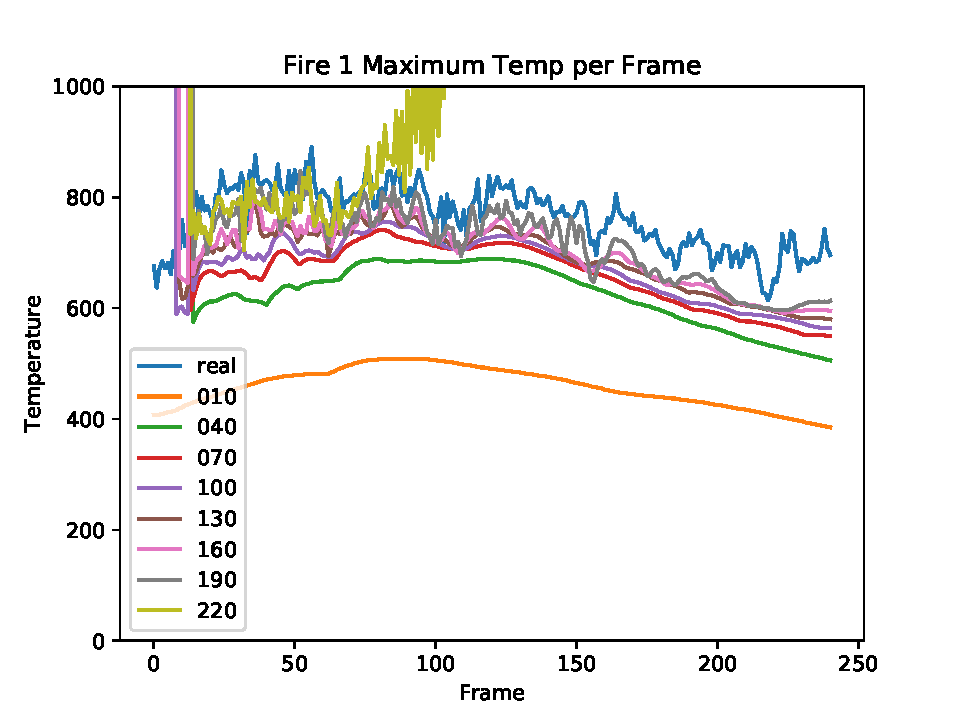
\includegraphics[width=1.1\linewidth]{../plots/f1_maxtemp.pdf} 
    \caption{Maximum temperature time series for Fire 1} 
    \vspace{4ex}
  \end{minipage}%%
  \begin{minipage}[b]{0.5\linewidth}
    \centering
    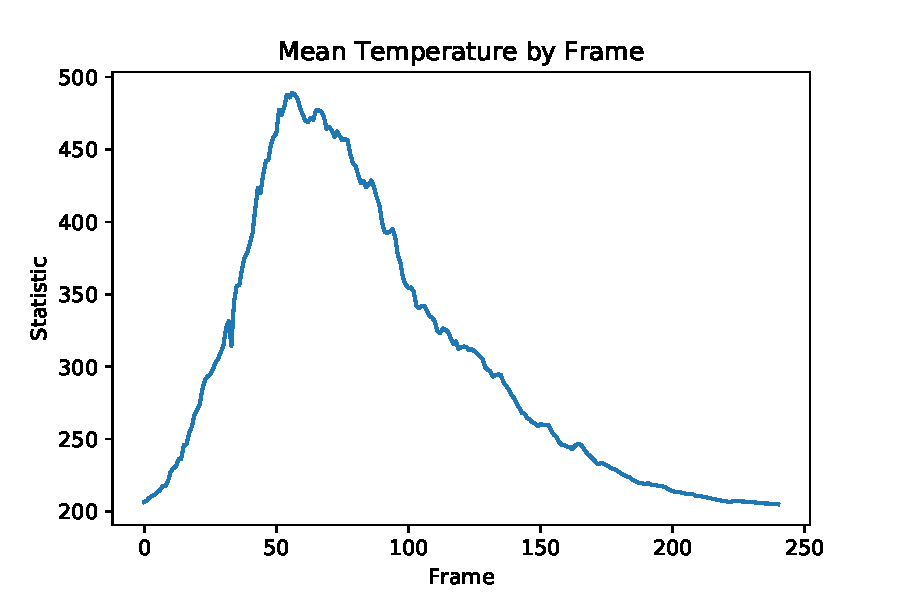
\includegraphics[width=1.1\linewidth]{../plots/f1_meantemp.pdf} 
    \caption{Mean temperature time series for Fire 1} 
    \vspace{4ex}
  \end{minipage} 
  \begin{minipage}[b]{0.5\linewidth}
    \centering
    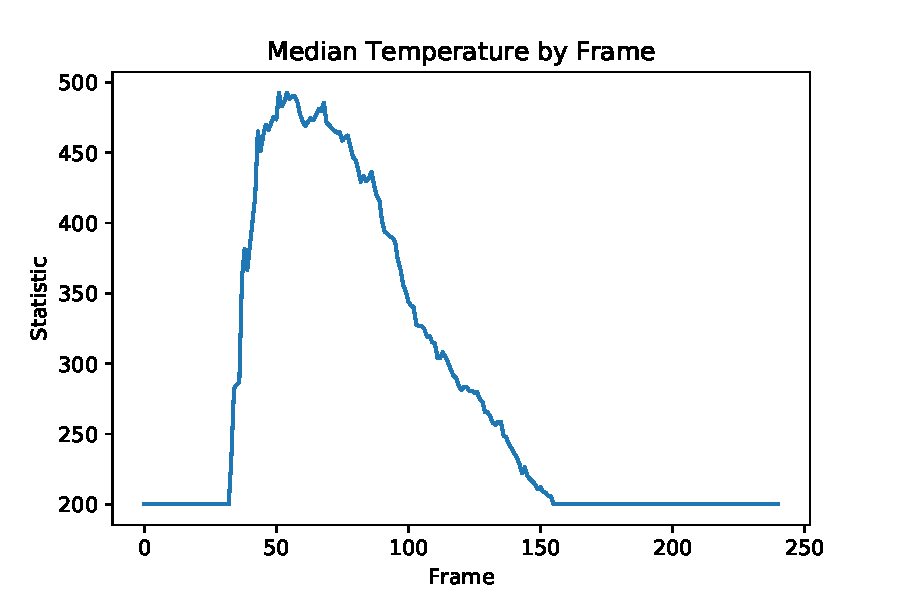
\includegraphics[width=1.1\linewidth]{../plots/f1_mediantemp.pdf} 
    \caption{Median temperature time series for Fire 1} 
    \vspace{4ex}
  \end{minipage}%% 
  \begin{minipage}[b]{0.5\linewidth}
    \centering
    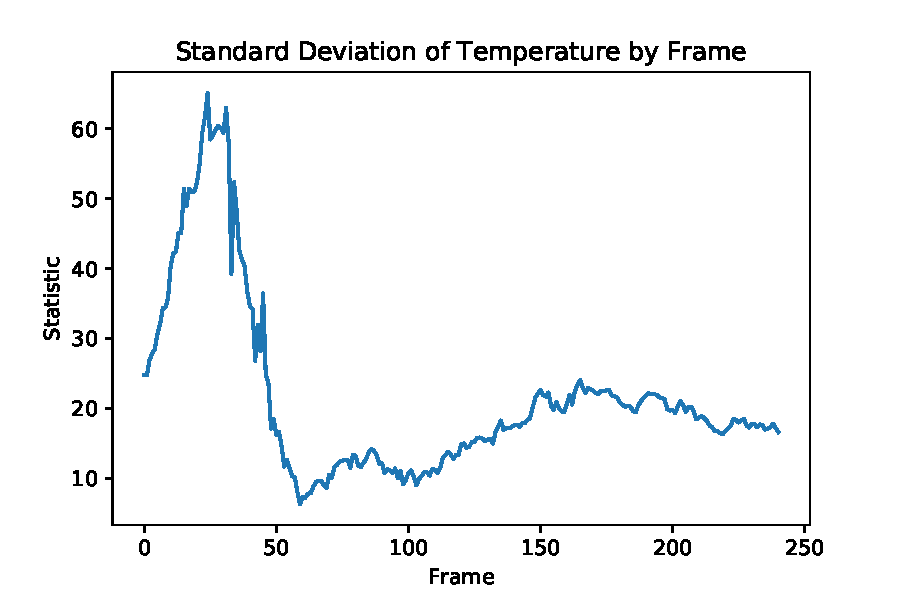
\includegraphics[width=1.1\linewidth]{../plots/f1_stdtemp.pdf} 
    \caption{Standard deviation time series for Fire 1} 
    \vspace{4ex}
  \end{minipage} 
\end{figure}


\pagebreak

\subsection{Fire 2}



\begin{table}
\centering
\begin{tabular}{|c|c|}
\hline
Data range used & Frames 9 through 200 \\
\hline 
Garbage Frames & None \\
\hline
\end{tabular} 


\caption{Good frames that were used in our analyses for Fire 2. No frames were thrown out die to read noise. Indexing begins at 1.}
\end{table}

\begin{figure}[ht] 
\centering
  \label{ fig7} 
  \begin{minipage}[b]{0.5\linewidth}
    \centering
    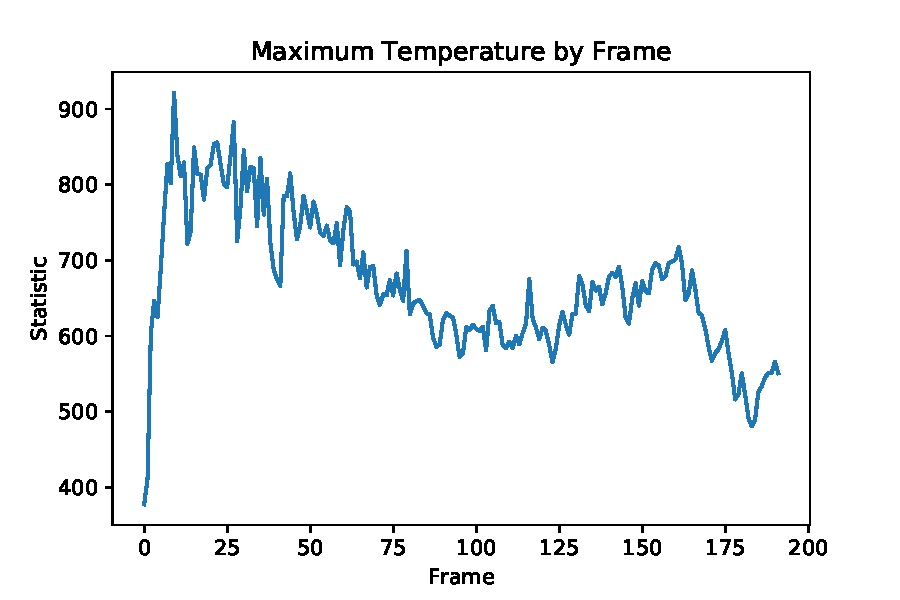
\includegraphics[width=1.1\linewidth]{../plots/f2_maxtemp.pdf} 
    \caption{Maximum temperature time series for Fire 2} 
    \vspace{4ex}
  \end{minipage}%%
  \begin{minipage}[b]{0.5\linewidth}
    \centering
    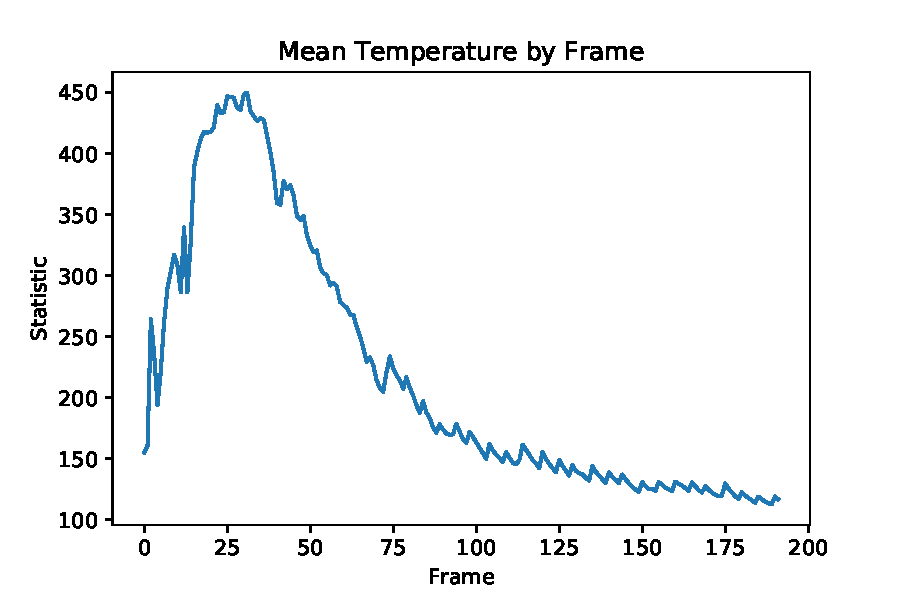
\includegraphics[width=1.1\linewidth]{../plots/f2_meantemp.pdf} 
    \caption{Mean temperature time series for Fire 2} 
    \vspace{4ex}
  \end{minipage} 
  \begin{minipage}[b]{0.5\linewidth}
    \centering
    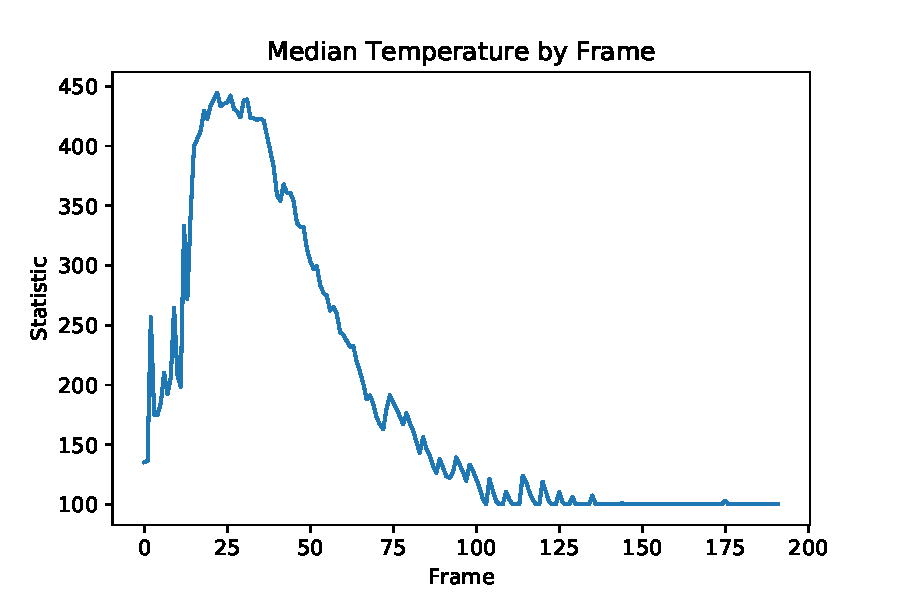
\includegraphics[width=1.1\linewidth]{../plots/f2_mediantemp.pdf} 
    \caption{Median temperature time series for Fire 2} 
    \vspace{4ex}
  \end{minipage}%% 
  \begin{minipage}[b]{0.5\linewidth}
    \centering
    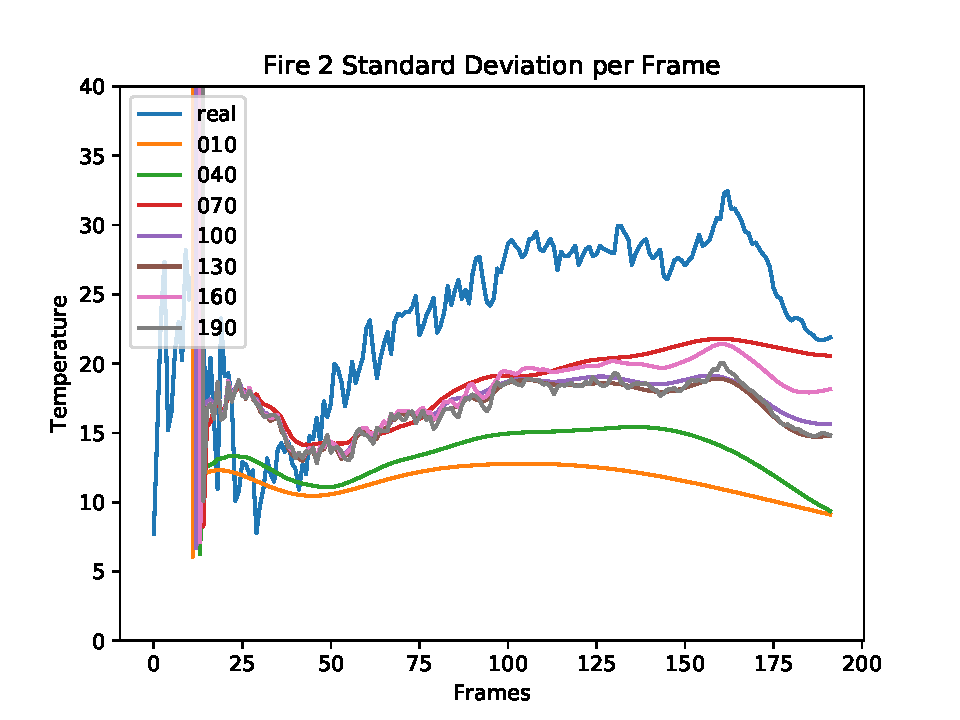
\includegraphics[width=1.1\linewidth]{../plots/f2_stdtemp.pdf} 
    \caption{Standard deviation time series for Fire 2} 
    \vspace{4ex}
  \end{minipage} 

\end{figure}

\pagebreak

\subsection{Fire 3}



\begin{table}
\centering
\begin{tabular}{|c|c|}
\hline
Data range used & Frames 45 through 220 \\
\hline 
Garbage Frames & 10, 30, 50, 71, 91, 112, 132, 152, 173, 213, \\
               & 233, 253, 273, 294, 314 \\

\hline
\end{tabular} 

\caption{Good frames that were used in our analyses for Fire 3 and frames that were thrown out due to significant read noise. Indexing begins at 1.}
\end{table}


\begin{figure}[ht] 
\centering
  \label{ fig7} 
  \begin{minipage}[b]{0.5\linewidth}
    \centering
    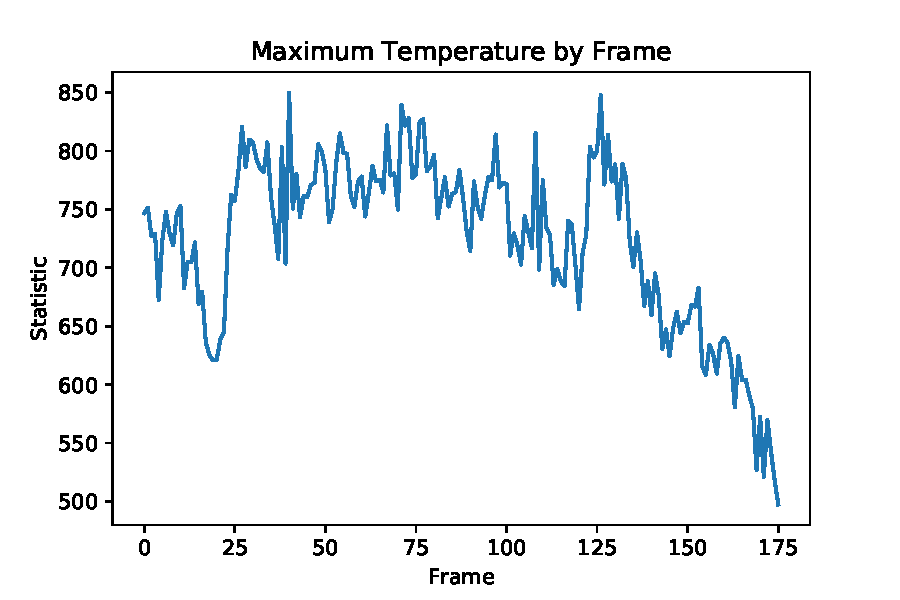
\includegraphics[width=1.05\linewidth]{../plots/f3_maxtemp.pdf} 
    \caption{Maximum temperature time series for Fire 3} 
    \vspace{4ex}
  \end{minipage}%%
  \begin{minipage}[b]{0.5\linewidth}
    \centering
    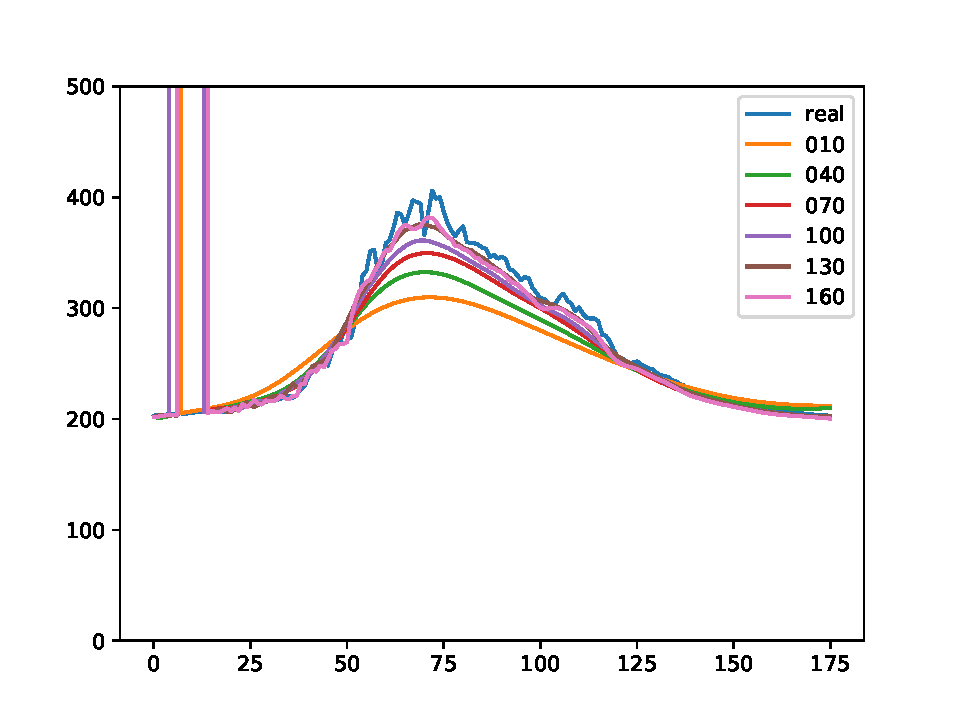
\includegraphics[width=1.05\linewidth]{../plots/f3_meantemp.pdf} 
    \caption{Mean temperature time series for Fire 3} 
    \vspace{4ex}
  \end{minipage} 
  \begin{minipage}[b]{0.5\linewidth}
    \centering
    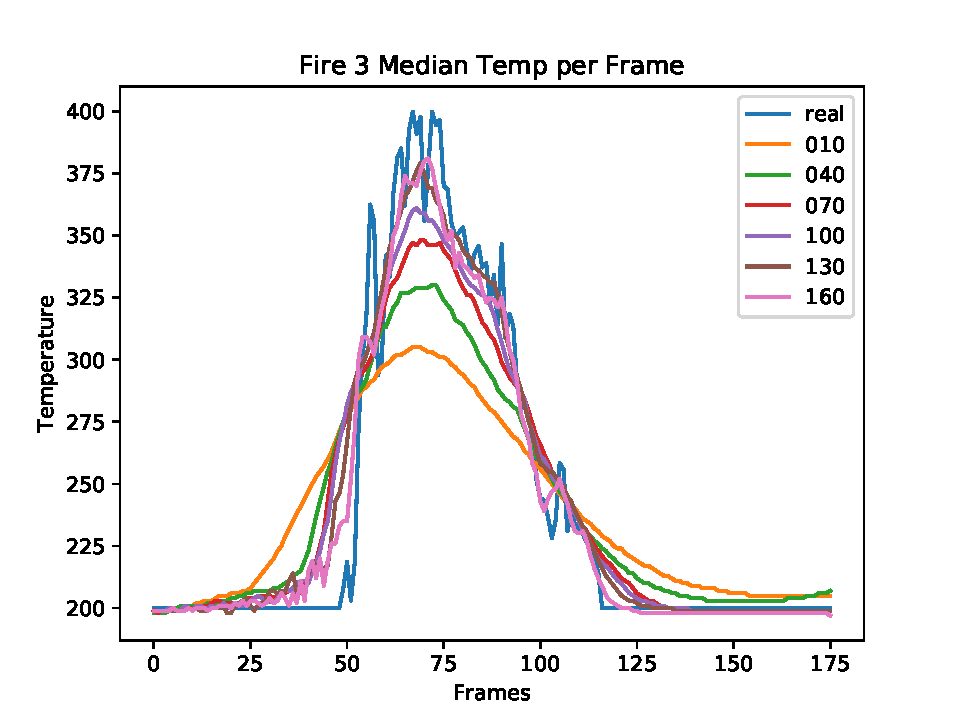
\includegraphics[width=1.05\linewidth]{../plots/f3_mediantemp.pdf} 
    \caption{Median temperature time series for Fire 3} 
    \vspace{4ex}
  \end{minipage}%% 
  \begin{minipage}[b]{0.5\linewidth}
    \centering
    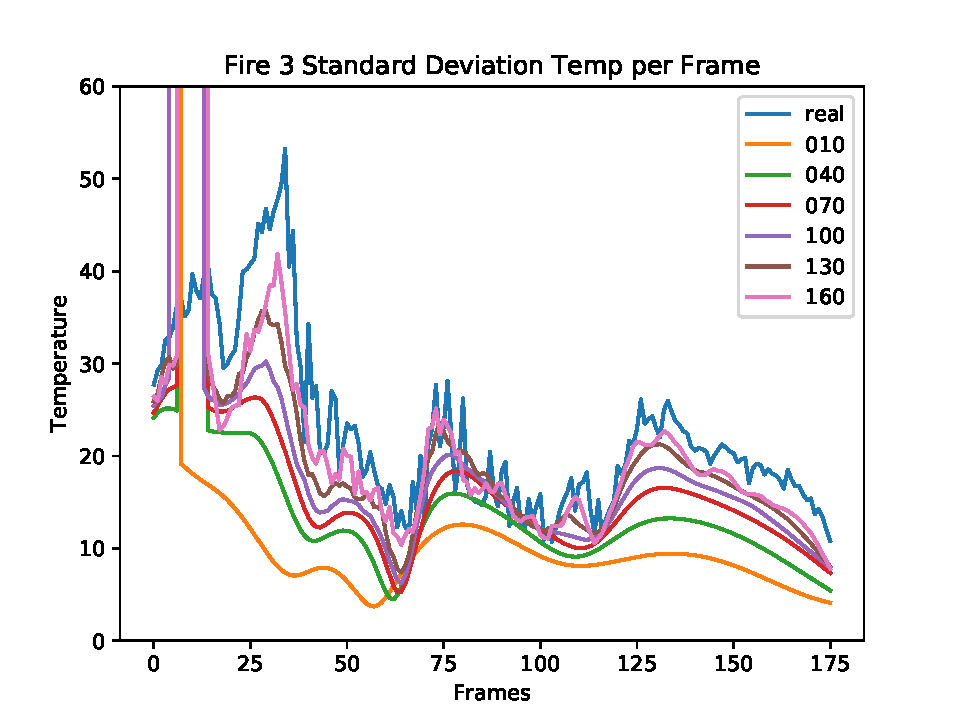
\includegraphics[width=1.05\linewidth]{../plots/f3_stdtemp.pdf} 
    \caption{Standard deviation time series for Fire 3} 
    \vspace{4ex}
  \end{minipage} 

\end{figure}

\section{Dynamic Mode Decomposition}


\begin{table}
\centering
\begin{tabular}{|c|c|c|c|c|c|c|c|c|}
\hline
Number of SVs & Max Temp & Min Temp & Mean Temp & Med Temp & Std Dev & Err Mean & Err Med & Err Std Dev \\
\hline
10 & 509.0 & 0 & 201.7 & 194.0 & 76.79 & 82.38 & 41.99 & 81.88 \\
\hline
40 & Inf & -2 & Inf & 214.0 & Inf & Inf & 15.37 & Inf \\
\hline
70 & Inf & -2 & Inf & 212.0 & Inf & Inf & 10.99 & Inf \\
\hline
100 & Inf & -2 & Inf & 210.0 & Inf & Inf & 9.75 & Inf \\
\hline
130 & Inf & -2 & Inf & 208.0 & Inf & Inf & 8.99 & Inf \\
\hline 
160 & Inf & -2 & Inf & 207.0 & Inf & Inf & 8.00 & Inf \\
\hline 
190 & Inf & -2 & Inf & 205.0 & Inf & Inf & 8.80 & Inf \\
\hline
220 & Inf & -Inf & Inf & 259.0 & Inf & Inf & 35.0 & Inf \\
\hline

\end{tabular}
\caption{hi this is a test}
\end{table}

\end{document}

